\section{Zaključek}
\label{sec:zakljuek}

V diplomskem delu smo najprej spoznali, da učenje računalniške
znanosti in programiranja spada v \textbf{primarno področje uporabe
  računalnika v izobraževanju}. Pri nas se je na splošnem
izobraževalnem področju uveljavila usmeritev, ki zagovarja
\textbf{splošno usposobljenost} za delo z računalnikom, kljub temu se
z računalniško znanostjo in programiranjem večina učencev prvič
srečaja pri izbirnih predmetih \emph{Urejanje besedil, Multimedija in
  Računalniška omrežja} in pri neobveznem izbirnem predmetu
\emph{Računalništva} v \textbf{OŠ}. Dijaki se srečajo s programiranjem
v 1. letniku pri predmetu \emph{Informatika}. Posebnost so strokovni
programi, katerim je osnova računalništvo in je poudarek na
programiranju dosti večji, kar smo spoznali pri pregledu učnega načrta
predmeta \emph{Računalništva} Tehniške gimnazije. Ugotovimo lahko da
je programiranje pri splošnih predmetih zastopano do te mere, da se
učenci oz. dijaki dotaknejo teh znanj, pri čemer je v bolj strokovnih
predmetih kot je pri \emph{Računalništvo} v OŠ in na programu Tehnični
gimnazije zastopano v vse podrobnosti.

Pri pregledu osnovnih pojmov smo spoznali kaj predstavljajo programske
paradigme in ugotovili, da danes prevladuje paradigma \textbf{objektno
  orientiranega} programiranja. Podrobneje smo predstavili značilnosti
programskih jezikov, ki so trenutno najbolj popularni in ti so
\textbf{Java, C++, JavaScript} in \textbf{Python}. Čeprav so v
slovenskem izobraževalnem prostoru na srednje šolskem nivoju prisotni
vsi omenjeni, se za začetnike priporoča uporaba \textbf{Python-a}. V
osnovni šoli bi se naj uporabljal programski jezik \textbf{Scratch},
ki uporablja grafičen način sestavljanja gradnikov. Pri spoznavanju
osnovnih konceptov programiranja smo pripravili nekaj primerov
programov, ki jih skušajo čim bolj nazorno predstaviti.

Pri proučevanju \textbf{aktivnega pristopa} smo spoznali, da pouk
računalništva mora biti pozitivno naravna in je naj znanje grajeno z
\textbf{aktivnim učenje}, torej učenci z lastnim delom odkrivajo in
gradijo miselni model. Pri tem so naj uporabljene
\textbf{konstruktivne metode} poučevanja. Za aktivno učenje je ravno
tako značilen problemsko naravnan pouk. Reševanje nalog
oz. raznovrstnih problemov je naravno prisoten pri poučevanju
računalniške znanosti, zato smo izpostavili \textbf{strategije
  reševanja problemov} in smo osnove korake podrobno
razdelali. Strategije reševanja problemov niso pomembne le za področje
računalništva temveč za mnoga področja tehničnih in znanstvenih
disciplin ter na sploh pri vsakdanjem življenju. Zanimalo nas ali so
vse te značilnosti pouka računalništva zajete tudi z uporaba spletnih
portalov.

Prvi spletni portali za učenje programiranja so nastali v akademskem
okolju na različnih univerzah po svet. Spoznali smo, da se študenti
novinci srečujejo vsepovsod s podobnimi težavami, kot je instalacija
in nastavitev programske opreme, uporaba IRO, uporaba sintakse
programskega jezika, razumevanje prevajalnika in tako
naprej. Pri vseh treh spletnih portalih, ki smo jih pregledali, smo
lahko strnili naslednje značilnosti, glavni del vsakega spletnega
portala je \textbf{spletna aplikacija za učenje programiranja
  (SAZP)}. Njene značilnosti so, da vsebuje \textbf{urejevalnik
  besedil, omogoča zagon napisanega programa, vrača povratne
  informacije o napakah ter izpis vhodno-izhodnih podatkov}. Drugi
elementi spletnega portala poleg SPZP so še \textbf{razdelane vsebine
  z nalogami, omogočena je komunikacija med mentorjem in novincem,
  omogočen je pregled nad napredkom novinca}.

Najzahtevnejši del tega diplomskega dela, je bilo iskanje kriterijev s
katerimi smo lahko spletne portale klasificirali in jih
ovrednotili. Najprej smo jih razdelili po vrsti vsebine in
ugotovili, da so najzanimivejše tiste vsebine, ki so
\textbf{kombinirane}. Kombinirane vrste vsebin smo razdelili na
\textbf{osnovne} in \textbf{napredne}, v slednjih se prepleta
\textbf{SPZP}, tekstovni ali/in video \textbf{vodiči} ter
\textbf{navodila}. Vsi ti elementi napredne kombinirane vsebine
tvorijo \textbf{vadnico}, ki je navadno osnovna enota neke učne teme.
Za posamezni spletni portal želimo določiti v katerem \textbf{jeziku}
je predstavljen, katera \textbf{znanja ponuja}, ali so to veščine
programiranja, znanja algoritmov, ali morda druga projektna znanja,
kot je izdelava spletne strani. Za vsak spletni portal smo zapisali,
učenje katerih \textbf{programskih jezikov} omogoča, kakšni
\textbf{težavnostni stopnji} je namenjen. Podrobneje so nas zanimala
ali spletni portali, tisti z vsebino znajo upoštevati nekatera
\textbf{učna načela}, kot je \textbf{problemski pristop, načelo
  sistematičnosti} in \textbf{načelo postopnosti}. Pri posameznem
spletnem portalu smo izpostavili ali ta uporablja \textbf{ocenjevanje,
dosežkov}, ki je značilno za video igre. Zanimalo nas je še ali
omogočajo spletni portali, da \textbf{dodajamo lastne vsebine} ter ali je
omogočeno \textbf{upravljanje razreda}. Nazadnje nas je zanimalo ali
so gradiva na spletnih portalih \textbf{brezplačna}, \textbf{pol
  plačljiva}, torej so nekatera gradiva ali storitve brezplačne druga
plačljiva in \textbf{popolnoma plačljive}.

Spletnih portalov, ki želijo poučevati računalniške znanosti in
programiranja je na spletu zarez veliko, zato smo morali določiti
omejitve s katerimi smo izbrali tiste, za katere smatramo, da nam bodo
pri pouku najbolj v pomoč. Te omejitve so naslednje, spletni portal
mora vsebovati \textbf{SAZP}, ki pa lahko nastopa tudi samostojno brez
vsebine, vrsta vsebin naj bo \textbf{kombinirana} ter naj bodo vsebine
na spletnih portalih dosegljive \textbf{brezplačno} ali \textbf{pol
  plačljivo}. Veliko spletnih portalov, ki na prvi pogled vabijo s
kvalitetno pripravljeno vsebino in vadnico, zaradi popolne
plačljivosti nismo mogli uvrstiti na seznam podrobne obravnave, saj
zaradi tega razloga niso uporabne za pouk.

V diagramu (slika \ref{fig:spup_povzetek}) smo zbrali povzetek
pregleda spletnih portalov. Portale smo razvrstili po vrsti
vsebine. Vsaki smo dodali predstavnike, ki smo jih pregledali, povzeli
smo skupne značilnosti vsake vrste in za posamezni portal pripisali
izstopajoče lastnosti.

\begin{figure}[h!]
  \centering
    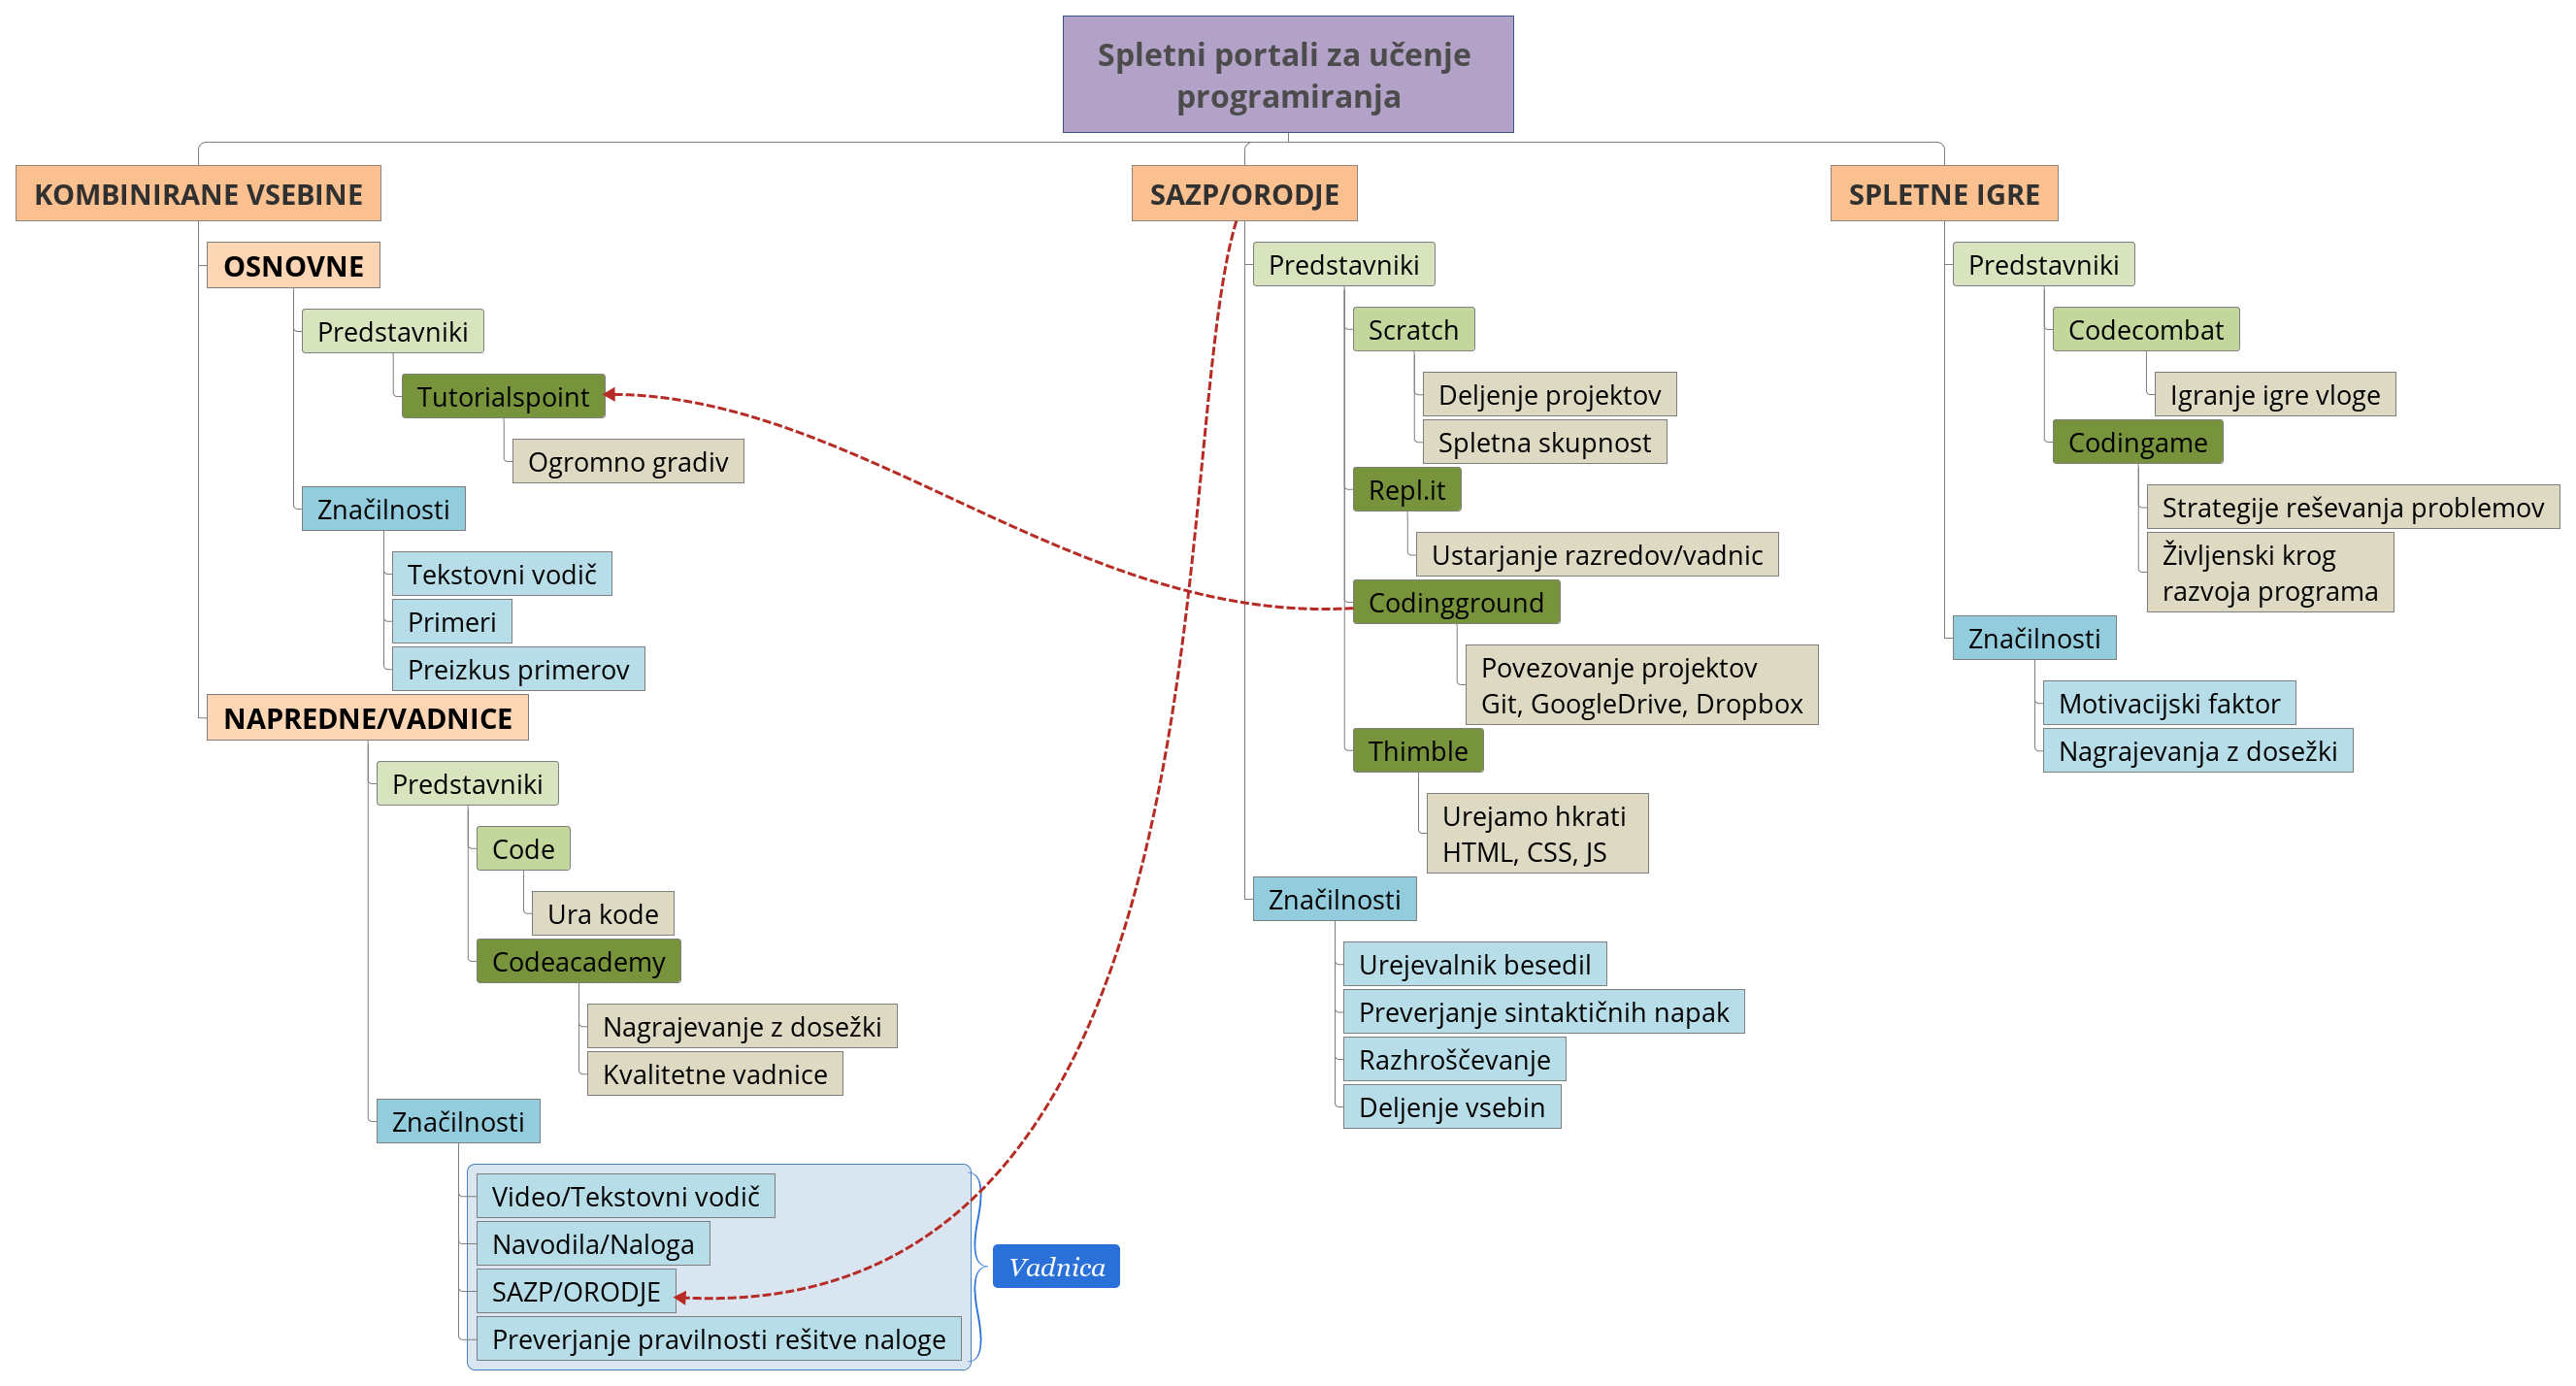
\includegraphics [width=1\linewidth, keepaspectratio =
   1] {./images/SPUP_povzetek-xmind.png}
   \caption{Miselni vzorec z povzetkom pregledanih spletnih portalov s
   predstavniki in značilnostmi za posamezno vrsto vsebine.}
 \label{fig:spup_povzetek}
\end{figure}
 
Najprej povzemimo spletne portale \textbf{Kombiniranih vsebin}, ti se
ponašajo s kvalitetno pripravljenimi \textbf{vadnicami}. Posamezni
vsebinski sklopi so razdeljeni na manjše enote, ki so med seboj
sistematično povezane. Taki spletni portali nudijo tudi ideje in
pripravljena gradiva za mentorje. Pregledali smo portal \emph{Code},
ki je uporaben predvsem za uvodne učne ure računalništva v OŠ tudi v
razredih prve triade. Spletni portal \emph{Codeacademy} je primeren
predvsem v SŠ kot dopolnilno gradivo učenja programskih jezikov kot je
\textbf{Python} in osnovnih konceptov programiranja. Glavna težava teh
portalov je ta, da so gradiva napisana v \textbf{angleškem
  jeziku}. Mentor mora v ta namen imeti pripravljene prevode navodil
nalog. Učne ure z uporabo teh spletnih portalov lahko uporablja z med
predmetno povezavo s predmetom Angleščina.

V posebno kategorijo smo uvrstili spletne portale, ki ponujajo
samostojno \textbf{spletno aplikacijo za programiranje}, ki jo
uporabimo kot orodje. Ti portali navadno ne vsebujejo lastnih
vsebin. Kot prvo smo pregledali spletni aplikacijo \textbf{Scrach}, ki
je v OŠ že dobro poznana. Scratch ima številne zmožnosti in bi ga
lahko uporabili takoj po uvodu, ki ga naredimo s spletnim portalom
\emph{Code}. Naslednja SAZP, \emph{Repl.it} omogoča ustvarjanje
razredov in lastnih vadnic. V vadnicah lahko vključimo teoretični
uvod, navodila, ter ogrodje programa. \emph{Codingground}, ki je del
spletnega portala \emph{Tutorials point} omogoča dober urejevalnik
besedil z ukazno vrstico ter dobro povezljivost z oblačnimi shrambami
kot je \textbf{Dropbox, GoogleDrive, OneDrive} in kontrolo verzije
\textbf{Git}. \emph{Thimble} omogoča ustvarjanje projektov, z večimi
ločenimi datotekami, projekt delimo naprej, tako da jih uporabniki ali
učenci lahko spreminjajo. Izkaže se za odlično orodje učenja spletnih
tehnologij. Bistvena prednost uporabe SAZP je ta, da ima mentor,
svobodno izbiro, katero vsebino bo podajal, vendar mora v priprava
vsebine vložiti več truda in časa. Vsebino prilagaja in jo prireja po
potrebi učnega načrta ter lastni presoji zmožnosti učencev.

Posebna kategorija spletnih portalov za učenje programiranja so
\textbf{spletne igre}. Izpostavili smo dve, prva \emph{Codecomba}, je
namenjena višjim razredom OŠ ter SŠ. Čeprav smo govorili o tem, da
pisani programski jeziki niso primerni za uporabo v OŠ ta spletni
portal predstavlja izjemo, kar smo povzeli s primerom možnih načinov
uporabe spletnih portalov. Spletna igra temelji na \textbf{igranju
  igre vloge}, igralec prevzame vlogo junaka, ki ga vodi in se z njim
bojuje s pisanjem programske kode. Junak ima omogočene veščine torej
metode programskega jezika, ki jih uporablja in so vgrajene v različne
predmete ali opremo. Drug primer spletne igre je \emph{Codingame}, ki
sodi v višjo zahtevnost in je namenjen predvsem tistim, ki želijo
svoje znanje in veščino programiranja, poznavanje programskega jezika
ter algoritmov izpopolniti z dokaj zahtevnimi problemsko zastavljenimi
nalogami. Z reševanjem nalog se uporabnik ne le v strategijah
reševanja problemov in pisanja algoritmov temveč tudi optimizaciji
napisanega algoritma. Spletna aplikacija prav tako uči življenjski
krog pisanja programa. Skupna značilnost spletnim igram je ta, da
imajo močan motivacijski faktor, ki je včasih zelo potreben, da
novinci ostanejo pri pisanju programske kode in reševanju
problemov.

V splošnem lahko trdimo, da je uporaba spletnih portalov za učenje
programiranja problemsko naravnana in v sami osnovi vzpodbuja
aktivnost učencev. Uporaba prinaša prednosti za mentorja in novince ko
je ta, da ni potrebe po instalaciji programske oprem, kar omogoča
kompatibilnost na številnih platformah, saj lahko spletno aplikacijo
naložimo v vsakem novodobnem brskalniku. Novince ni potrebno priučiti
uporabe zahtevnih uporabniških vmesnikov IRO. Navadno je vsebina
spletnih portalov nastavljena tako, da jim ni potrebno pisati celotne
programske kode, saj je ogrodje že podano in morajo napisati samo
zahtevno rešitev. Tako se lahko bolje osredotočimo na reševanje
problemov. Kot smo v diplomskem delu spoznali so spletni portali za
učenje programiranja uporabni, vsak od njih ima svojo prednost. Na
mentorju je naloga, da čim bolj skuša izkoristiti te prednosti in s
tem poskuša navdušiti čim več novincev, da bodo postali dobri
programerji.

% V prihodnje bi morda bilo zanimivo raziskati koliko se spletni portali
% za učenje programiranja uporabljajo pri nas in kakšen portal bi si
% želeli učitelji, da bi lažje poučevali računalništvo 

 %%% Local Variables:
 %%% mode: latex
 %%% TeX-master: "../diploma"
 %%% End:
